\documentclass{standalone}
\usepackage{pgfplots}
\pgfplotsset{compat=1.13}
\usepackage{amsmath}
\colorlet{paleBlue}{blue!10!white}

\begin{document}

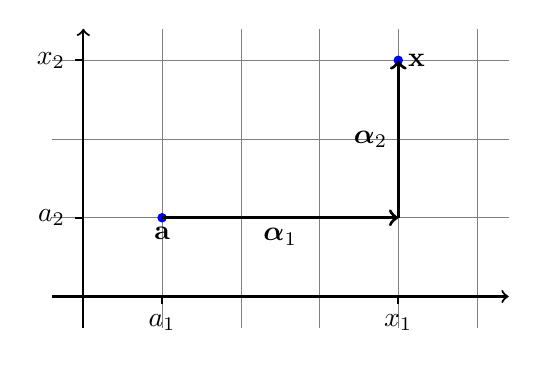
\begin{tikzpicture}
    \draw[step=1cm,gray,very thin] (-0.4,-0.4) grid (5.4,3.4);
    \draw[thick,->] (-0.4,0) -- (5.4,0);
    \draw[thick,->] (0,-0.4) -- (0,3.4); 
    \draw[fill, blue] (1,1) circle [radius=1.5pt];
    \node[below] at (1,1) {\(\mathbf{a}\)};
    \draw[fill, blue] (4,3) circle [radius=1.5pt];
    \node[right] at (4,3) {\(\mathbf{x}\)};
    \draw[->, very thick] (1,1) -- (4,1) node[black,midway,below]{\(\boldsymbol{\alpha}_1\)};
    \draw[->, very thick] (4,1) -- (4,3) node[black,midway,left]{\(\boldsymbol{\alpha}_2\)};
    \draw[thick] (1,0) -- (1,-.1) node[below] {\(a_1\)};
    \draw[thick] (4,0) -- (4,-.1) node[below] {\(x_1\)};
    \draw[thick] (0,1) -- (-.1,1) node[left] {\(a_2\)};
    \draw[thick] (0,3) -- (-.1,3) node[left] {\(x_2\)};
\end{tikzpicture}

\end{document}